\subsection{Unterquadrate}
\label{sec:unterquadrate}

\begin{figure}[H]
    \centering
    \begin{minipage}{0.48\textwidth}
            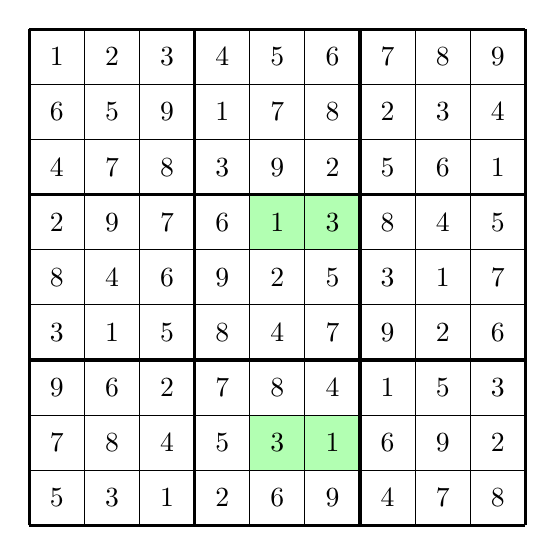
\begin{tikzpicture}
                % Zellgröße
                \def\s{0.7cm}

                % Sudoku-Lösung (kann beliebig angepasst werden)
                \def\sudoku{
                        {1, 2, 3, 4, 5, 6, 7, 8, 9},
                        {6, 5, 9, 1, 7, 8, 2, 3, 4},
                        {4, 7, 8, 3, 9, 2, 5, 6, 1},
                        {2, 9, 7, 6, 1, 3, 8, 4, 5},
                        {8, 4, 6, 9, 2, 5, 3, 1, 7},
                        {3, 1, 5, 8, 4, 7, 9, 2, 6},
                        {9, 6, 2, 7, 8, 4, 1, 5, 3},
                        {7, 8, 4, 5, 3, 1, 6, 9, 2},
                        {5, 3, 1, 2, 6, 9, 4, 7, 8},
                }

                \fill[green!30] (5*\s, 5*\s) rectangle (6*\s, 6*\s);
                \fill[green!30] (4*\s, 5*\s) rectangle (5*\s, 6*\s);

                \fill[green!30] (5*\s, 1*\s) rectangle (6*\s, 2*\s);
                \fill[green!30] (4*\s, 1*\s) rectangle (5*\s, 2*\s);

                % Rasterlinien
                \foreach \x in {0,1,...,9} {
                    \draw[thin] (\x*\s, 0) -- (\x*\s, 9*\s);
                    \draw[thin] (0, \x*\s) -- (9*\s, \x*\s);
                }
                \foreach \x in {0,3,6,9} {
                    \draw[very thick] (\x*\s, 0) -- (\x*\s, 9*\s);
                    \draw[very thick] (0, \x*\s) -- (9*\s, \x*\s);
                }




                % Zahlen eintragen
                \foreach \row [count=\i from 0] in \sudoku {
                    \foreach \num [count=\j from 0] in \row {
                    % Y-Koordinate: Startet oben bei 8.5 und geht pro Zeile 1 runter
                        \node at (\j*\s + 0.5*\s, 8.5*\s - \i*\s) {\num};
                    }
                }
            \end{tikzpicture}
    \end{minipage}
    \hfill
    \begin{minipage}{0.48\textwidth}
            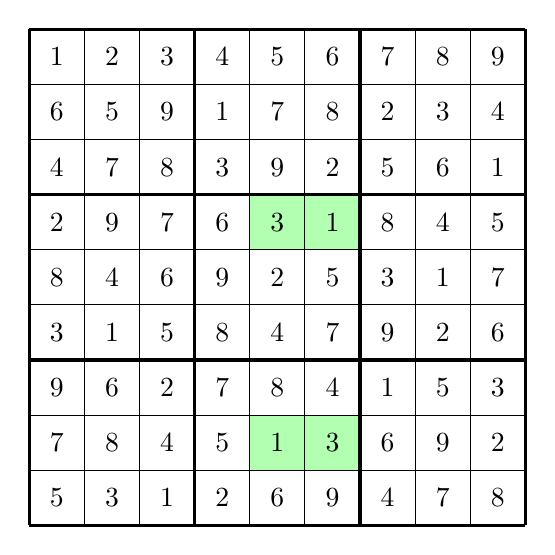
\begin{tikzpicture}
                % Zellgröße
                \def\s{0.7cm}

                % Sudoku-Lösung (kann beliebig angepasst werden)
                \def\sudoku{
                        {1, 2, 3, 4, 5, 6, 7, 8, 9},
                        {6, 5, 9, 1, 7, 8, 2, 3, 4},
                        {4, 7, 8, 3, 9, 2, 5, 6, 1},
                        {2, 9, 7, 6, 3, 1, 8, 4, 5},
                        {8, 4, 6, 9, 2, 5, 3, 1, 7},
                        {3, 1, 5, 8, 4, 7, 9, 2, 6},
                        {9, 6, 2, 7, 8, 4, 1, 5, 3},
                        {7, 8, 4, 5, 1, 3, 6, 9, 2},
                        {5, 3, 1, 2, 6, 9, 4, 7, 8},
                }

                \fill[green!30] (5*\s, 5*\s) rectangle (6*\s, 6*\s);
                \fill[green!30] (4*\s, 5*\s) rectangle (5*\s, 6*\s);

                \fill[green!30] (5*\s, 1*\s) rectangle (6*\s, 2*\s);
                \fill[green!30] (4*\s, 1*\s) rectangle (5*\s, 2*\s);

                % Rasterlinien
                \foreach \x in {0,1,...,9} {
                    \draw[thin] (\x*\s, 0) -- (\x*\s, 9*\s);
                    \draw[thin] (0, \x*\s) -- (9*\s, \x*\s);
                }
                \foreach \x in {0,3,6,9} {
                    \draw[very thick] (\x*\s, 0) -- (\x*\s, 9*\s);
                    \draw[very thick] (0, \x*\s) -- (9*\s, \x*\s);
                }




                % Zahlen eintragen
                \foreach \row [count=\i from 0] in \sudoku {
                    \foreach \num [count=\j from 0] in \row {
                    % Y-Koordinate: Startet oben bei 8.5 und geht pro Zeile 1 runter
                        \node at (\j*\s + 0.5*\s, 8.5*\s - \i*\s) {\num};
                    }
                }
            \end{tikzpicture}
    \end{minipage}
    \caption{Gemeinsame Beschriftung für beide Sudoku-Gitter}
    \label{fig:gemeinsames_sudoku}
\end{figure}

Innerhalb von vollständig ausgefüllten Sudokus kann es Unterquadrate geben.
Ein Beispiel für ein solches Unterquadrat ist in \cref{fig:gemeinsames_sudoku} gegeben.
Ein Unterquadrat besteht aus vier Zellen in denen zwei Ziffern jeweils doppelt vorkommen.
Je zwei Zellen sind dabei in der gleichen Spalte beziehungsweise in der gleichen Zeile.
Entweder beide Zeilen oder beide Spalten sind im gleichen Band.
Durch die Anordnung der Zellen ist es möglich, ein weiteres gültiges Sudoku zu generieren, nur durch Permutieren der beiden Ziffern im Unterquadrat.
Das bedeutet, dass ein partielles Sudoku, welches ein vollständiges Sudoku mit Unterquadrat als Lösung hat, nicht eindeutig lösbar ist,
wenn in keinem der Zellen der Unterquadrats eine Ziffer vorgegeben ist.